\documentclass[10pt,ngerman]{beamer}

\usepackage[ngerman]{babel}

\usepackage{csquotes}

\usetheme[progressbar=frametitle]{metropolis}
\usepackage{appendixnumberbeamer}

\usepackage[utf8]{inputenc}

\usepackage[bibencoding=utf8,sortlocale=de_DE,style=footnote-dw,ibidpage=true,origfieldsformat=brackets,backend=biber]{biblatex}
\addbibresource{Literaturverzeichnis.bib}
\renewcommand\bibname{Literaturverzeichnis}

\usepackage{booktabs}
\usepackage[scale=2]{ccicons}

\usepackage{xcolor, soul}
\definecolor{codebackground}{rgb}{0.95, 0.95, 0.92}
\definecolor{Black}{rgb}{0, 0, 0}


\usepackage{graphicx}

\usepackage{siunitx}
\sisetup{
  locale = DE ,
  detect-all,
  binary-units = true
}

\usepackage{listings}
\lstdefinestyle{MyLatexStyle} {
  frame=tb, % hrule above and below
  keepspaces=true,
  breaklines=true,
  columns=flexible,
  basicstyle=\tt\scriptsize,
  escapeinside={(*@}{@*)}, 
  backgroundcolor=\color{codebackground},
  showstringspaces=false,% for escapin
  language=[LaTeX]TeX,
  keywordstyle=\color{blue},
  identifierstyle=\color{magenta},
  stringstyle=\color{red},
  commentstyle=\color{teal},
  gobble=4
}
\lstdefinestyle{MyPythonStyle}{
  frame=tb, % hrule above and below
  keepspaces=true,
  breaklines=true,
  columns=flexible,
  basicstyle=\tt\scriptsize,
  escapeinside={(*@}{@*)}, % for escaping
  backgroundcolor=\color{codebackground},
  showstringspaces=false,
  language=Python,
  keywordstyle=\color{blue},
  stringstyle=\color{red},
  commentstyle=\color{teal},
  numbers=left, % {none, left, right}
  firstnumber=1,
  numberstyle=\scriptsize\color{black},
  numbersep=5pt,
  xleftmargin=5.0ex,
  gobble=4
}

\lstset{literate=%
    {Ö}{{\"O}}1
    {Ä}{{\"A}}1
    {Ü}{{\"U}}1
    {ß}{{\ss}}1
    {ü}{{\"u}}1
    {ä}{{\"a}}1
    {ö}{{\"o}}1
    {~}{{\textasciitilde}}1
}

\usepackage{caption}

%%% Für Quotes %%%
\usepackage{url}
\usepackage[ngerman]{varioref}
\usepackage{hyperref}
\setlength{\parindent}{0em}
\usepackage{cleveref}
\crefname{paragraph}{Abschnitt}{Abschnitt}

\usepackage{xspace}
\newcommand{\themename}{\textbf{\textsc{metropolis}}\xspace}
\definecolor{mSybilaRed}{HTML}{990000}

\setbeamercolor{title separator}{
  fg=mSybilaRed
}

\setbeamercolor{progress bar}{%
  fg=mSybilaRed,
  bg=mSybilaRed!90!black!30
}

\setbeamercolor{progress bar in section page}{
  use=progress bar,
  parent=progress bar
}

\setbeamercolor{alerted text}{%
  fg=mSybilaRed
}

\title{Projektpräsentation}

% \titlegraphic{\hfill
\includegraphics[height=2.5cm]{pictures/python-logo.png}}

%\titlegraphic{\hfill\includegraphics[height=2.5cm]{pictures/LaTeX_logo.png}}
%\titlegraphic{\hfill\includegraphics[height=0.6cm]{sybila-logo/new.png}}
%\titlegraphic{\hfill\includegraphics[height=0.6cm]{sybila-logo/old.png}}
%\titlegraphic{\hfill\includegraphics[height=0.6cm]{sybila-logo/old-flat.png}}

\date{12.05.2022}
\author{Julius Caesar, Péter Egermann, Paul Görtler, Johannes Leyrer}
\institute{BSZ für Elektrotechnik Dresden -- IT20/2}

\subtitle{Die hard- und softwaretechnische Implementierung eines CO$_2$-Sensors zur Messung der Raumluftqualität}
%\institute{Center for modern beamer themes}
% \titlegraphic{\hfill\includegraphics[height=1.5cm]{logo.pdf}}

\setbeamertemplate{footline}
{
  \leavevmode
  \hbox{
  \begin{beamercolorbox}[wd=.15\paperwidth,ht=2.25ex,dp=1ex,center]{title in head/foot}
    \usebeamerfont{author in head/foot} % \insertshortauthor
  \end{beamercolorbox}

  \begin{beamercolorbox}[wd=.7\paperwidth,ht=2.25ex,dp=1ex,center]{author in head/foot}
    \usebeamerfont{author in head/foot}\insertshorttitle
  \end{beamercolorbox}

  \begin{beamercolorbox}[wd=.15\paperwidth,ht=2.25ex,dp=1ex,center]{title in head/foot}
    \insertframenumber{} / \inserttotalframenumber
  \end{beamercolorbox}
  }
}

\begin{document}

\maketitle

\begin{frame}{Gliederung}
  \setbeamertemplate{section in toc}[sections]
  \tableofcontents[hideallsubsections]
\end{frame}

\section{Einleitung zum Vortrag PETER}

\section{Einleitung zum Projekt PETER}

\section{CO2-Grenzwerte nach DGUV PETER}

\section{Auswirkungen von zum hohem CO2-Gehalt PETER}

\section{Hardwaretechnische Umsetzung JULIUS}

\section{Softwaretechnische Umsetzung}

\subsection{Grundlagen}
\begin{frame}[fragile]{Grundlagen}
    \begin{minipage}[t]{0.49\textwidth}
      \begin{itemize}
        \item Linux-Distribution inklusive mitgelieferter Standardsoftware
        \item Docker
        \item Python
        \item FastAPI
        \item React
        \item ChartJs
        \item SQLite
      \end{itemize}
    \end{minipage}
    \begin{minipage}[t]{0.49\textwidth}
      \begin{figure}
        \centering
        \captionsetup{justification=centering}
        
\includegraphics[width=1\textwidth]{pictures/SoftwareKomponenten.png}
        \caption{Verwendete Softwarekomponenten}
      \end{figure}
    \end{minipage}
\end{frame}

\subsection{Zusammenspiel der Softwarekomponenten}

\begin{frame}[fragile]{Zusammenspiel der Softwarekomponenten}

  \begin{minipage}[t]{0.29\textwidth}
    \begin{itemize}
      \item Backend
      \item Frontend
      \item Datenbank
      \item Lese-Software
      \item[$\rightarrow$] Docker
    \end{itemize}
  \end{minipage}
  \begin{minipage}[t]{0.69\textwidth}
    \begin{figure}
      \centering
      \captionsetup{justification=centering}
      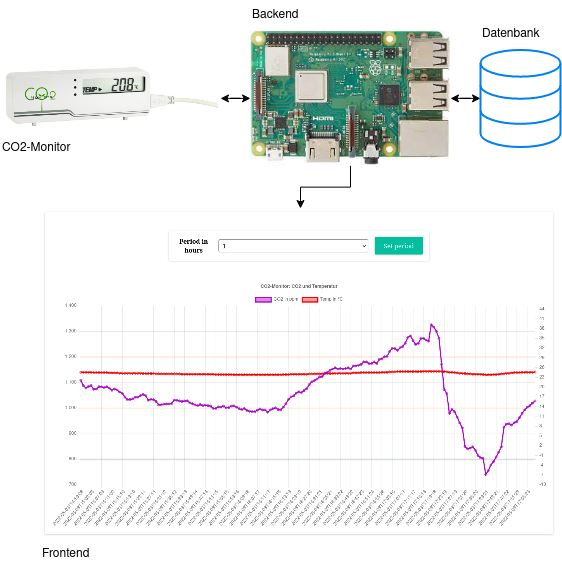
\includegraphics[width=170px]{pictures/SoftwareZusammenspiel.png}
      \caption{Zusammenspiel der Softwarekomponenten}
    \end{figure}
  \end{minipage}
\end{frame}

\subsection{Aufbau und Einrichtung der Softwarekomponenten JOHANNES}

\begin{frame}[fragile]{Aufbau und Einrichtung der Softwarekomponenten}

  \begin{minipage}[t]{0.49\textwidth}
    \begin{itemize}
      \item Backend: Python mit FastAPI
      \item Frontend: React und ChartsJs
      \item Lese-Software: Python-Script
      \item Datenbank: SQLite
    \end{itemize}
  \end{minipage}

  \begin{lstlisting}[language=Bash]
    docker-compose -f docker-compose.yml up -d
  \end{lstlisting}
\end{frame}

\section{Fazit}
\begin{frame}[fragile]{Fazit}
  \begin{minipage}[t]{0.80\textwidth}
    \textbf{Ergebnisse:}\newline
    \begin{itemize}
      \item bestätigte Relevanz der Raumluftqualität
      \item bestätigte Verbindung zwischen hohen CO$_2$-Konzentrationen und verminderter Konzentrationsfähigkeit/Produktivität
      \item schaffen einer kostengünstigen Möglichkeit zur selbstständigen Kontrolle der Raumluftqualität
    \end{itemize}
  \end{minipage}
\end{frame}


% \section{Geschichte}

% \begin{frame}[fragile]{Geschichte\footcite{wiki:python}}

%   \begin{minipage}[t]{0.69\textwidth}
%     \begin{itemize}
%       \item Entwickler: Guide van Rossum
%       \item Erscheinungsjahr: 20. Februar 1991
%       \item Name bezieht sich auf die Komikergruppe Monty Python
%       \item Open-Source
%       \item Python 2.0: 16. Oktober 2000 (Garbage Collection, Unicode)
%       \item Python 3.0: 03. Dezember 2008
%     \end{itemize}
%   \end{minipage}
%   \begin{minipage}[t]{0.29\textwidth}
%     \begin{figure}
%       \centering
%       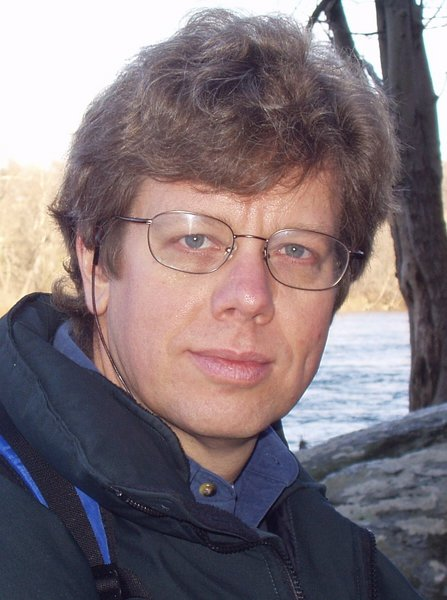
\includegraphics[width=0.9\textwidth]{pictures/Guido_van_Rossum.jpg}
%       \caption[Guido van Rossum, https://upload.wikimedia.org/wikipedia/commons/c/c6/Guido_van_Rossum.jpg, abgerufen am 16.11.2021 ]{Guido van Rossum, Entwickler von Python}
%     \end{figure}
%   \end{minipage}
% \end{frame}

% \section{Grundlagen}

% \begin{frame}[fragile]{Basiscs\footcite{wiki:python}}
%   \begin{itemize}
%     \item Beliebteste Programmiersprache laut PYPL-Index (PopularitY of Programming Language, Stand: November 2021)
%     \item universelle, interpretierte, höhere Programmiersprache
%     \item Anspruch: gut lesbarer, knapper Programmierstil
%     \item Sehr Anfängerfreundlich
%     \item Multiparadigmensprache: OOP oder funktional
%     \item Blöcke durch Einrückungen
%     \item als Datei oder Notebook angelegt
%   \end{itemize}
% \end{frame}

% \begin{frame}[fragile]{Ranking: Beliebtheit von Programmiersprachen}
%   \begin{figure}
%     \centering
%     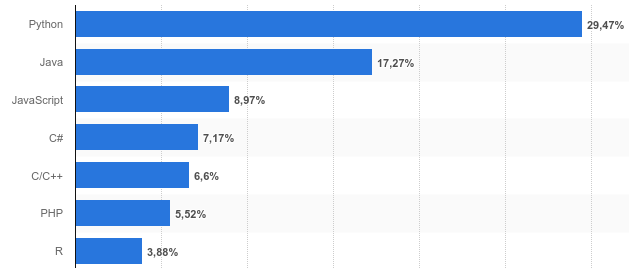
\includegraphics[width=1\textwidth]{pictures/statista_ranking.png}
%     \caption[Beliebtesten Programmiersprachen, https://de.statista.com/statistik/daten/studie/678732/umfrage/beliebteste-programmiersprachen-weltweit-laut-pypl-index/\#professional, abgerufen am 16.11.2021 ]{Die beliebtesten Programmiersprachen weltweit laut PYPL-Index im November 2021}
%   \end{figure}
% \end{frame}

% \begin{frame}[fragile]{Firmenbeispiele}
%   \begin{figure}
%     \centering
%     
\includegraphics[width=0.9\textwidth]{pictures/who_uses_python.png}
%     \caption[Weltweit agierende Firmen, die Python nutzen, https://www.monocubed.com/companies-that-use-python/, abgerufen am 16.11.2021 ]{Weltweit agierende Firmen, die Python nutzen}
%   \end{figure}
% \end{frame}

% \begin{frame}[fragile]{Hauptverwendungszwecke\footcite{coursera:pythonPopularity}}
%   \begin{itemize}
%     \item Sever Side Applications
%     \item Automatisierung von Aufgaben und Scripting
%     \item Big Data: Datenanalyse
%     \item Machine learning
%     \item Softwaretests und Prototyping
%   \end{itemize}
% \end{frame}

% \section{Nutzung und Beispiele}

% \begin{frame}[fragile]{.py vs .ipynb}

%   \begin{figure}
%     \centering
%     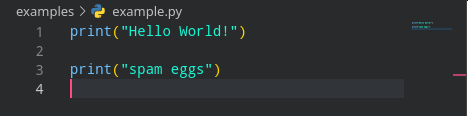
\includegraphics[width=0.7\textwidth]{pictures/py.png}
%     \caption[Beispiel einer .py-Datei]{Beispiel einer .py-Datei}
%   \end{figure}
%   \begin{figure}
%     \centering
%     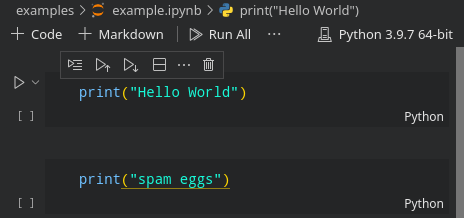
\includegraphics[width=0.7\textwidth]{pictures/ipynb.png}
%     \caption[Beispiel einer .ipynb-Datei]{Beispiel einer .ipynb-Datei}
%   \end{figure}
% \end{frame}

% \begin{frame}[fragile]{Codebeispiele}
%   \begin{figure}
%     \centering
%     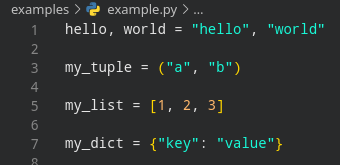
\includegraphics[width=0.9\textwidth]{pictures/examples.png}
%     \caption[Code-Beispiele]{Code-Beispiele}
%   \end{figure}
% \end{frame}

% \begin{frame}[fragile]{Codebeispiele}
%   \begin{figure}
%     \centering
%     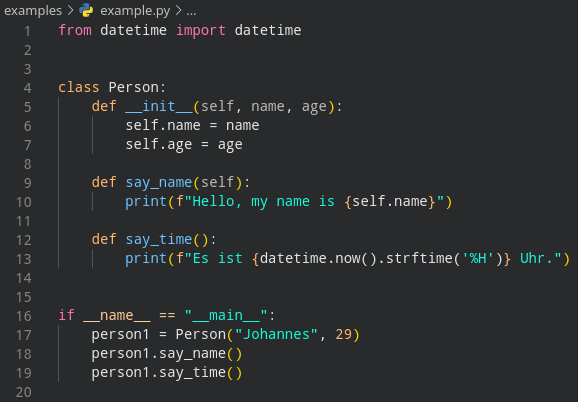
\includegraphics[width=0.9\textwidth]{pictures/class_example.png}
%     \caption[Code-Beispiel einer Klasse]{Code-Beispiel einer Klasse}
%   \end{figure}
% \end{frame}

% \begin{frame}[fragile]{Beliebtesten Libraries}
%   \begin{figure}
%     \centering
%     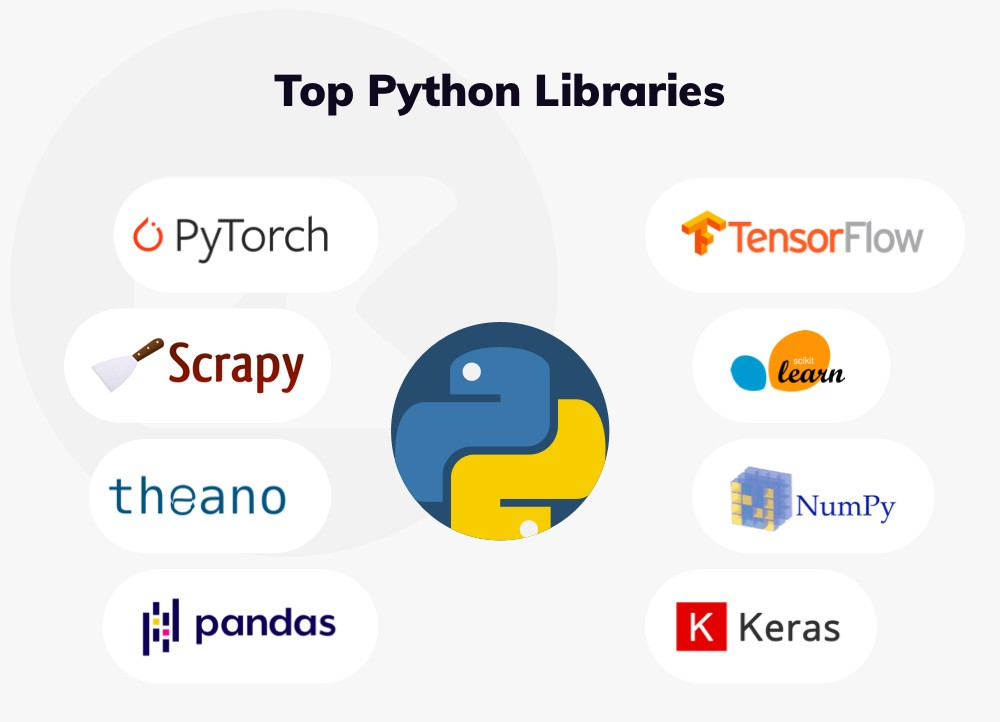
\includegraphics[width=0.8\textwidth]{pictures/libraries.jpg}
%     \caption[Beliebtesten Libraries in Python]{Beliebtesten Libraries in Python}
%   \end{figure}
% \end{frame}

\begin{frame}[standout]
  Fragen?
\end{frame}

\appendix

\begin{frame}[allowframebreaks]{Literaturverzeichnis}

  \printbibliography[title={Literaturverzeichnis}]

\end{frame}

\begin{frame}[standout]
  Danke für die Aufmerksamkeit!
\end{frame}
\end{document}
